\chapter{Background}
\label{chap:background}
\section{VEX System}
asd
\subsection{Architecture}
asd
\subsection{ISA}
asd
\subsection{Registers}
asd
\subsection{Run-time architecture}
asd

\section{LLVM Compiler infrastructure}
LLVM is based on the classic three-stage compiler architecture shown in figure \ref{fig:compiler_structure}. The compiler uses a number language specific front-ends, an optimizer and target specific backends. This modular design enables compiler designers to work on different parts of the compiler as a separate part. Support for a new processor can be added by building a new back-end. The existing front-end and optimizer can be reused for the new compiler.

\begin{figure}[ph!]
\centering
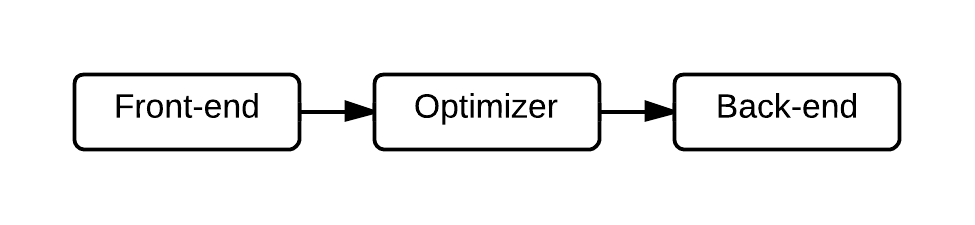
\includegraphics[width=0.8\textwidth]{2_background/img/Basic_compiler.png}
\caption{Basic compiler structure}
\label{fig:compiler_structure}
\end{figure}

The front-end is used to transform the plain text source code of a program into an intermediate representation that will be used during compilation process. This transformation is achieved by performing the following steps:

\begin{enumerate}
	\item \textbf{Lexical analysis:} Break input into individual tokens.
	\item \textbf{Syntax analysis:} Using a grammer the sequence of tokens is transformed into a parse tree which represents the structure of the program.
	\item \textbf{Semantic analysis:} Semantic information is added to the parse tree, type checking is performed and a symbol table is built.
\end{enumerate}

The resulting abstract syntax tree (AST) is transformed into LLVM IR and passed to the optimizer and backend of the compiler. These parts of the compilation process are completely language agnostic and do not require any other information from the front-end.

The optimizer is used to analyze and optimize the program. Optimization such as dead code elimination and copy propagation are performed during this phase but also more advanced operations that extract ILP (loop vectorization) can be enabled.

The back-end optimizes and generates code for a specific architecture. The LLVM IR is transformed into processor specific assembly instructions, allocates registers and schedules code for better performance.

\subsection{LLVM}
asd
\subsubsection{Front-end}
The modular design of LLVM enables the compiler to be used as a part of the existing GCC compiler. For example, the dragonegg GCC plugin is designed to replace the GCC code generator and optimizer with the LLVM backend. This would enable LLVM to be able to use the existing GCC based front-ends and supported languages.

Clang has been developed to allow LLVM to operate independently of GCC. Clang is a front-end supporting C, C++ and ObjC. The front-end is designed to be closely integrated with the Integrated Development Environment (IDE) allowing more expressive diagnostic messages. In addition Clang also aims to provide faster compilation and lower memory usage \cite{clang:features}.
\subsubsection{LLVM IR}
The front-end transforms a source code into the LLVM internal representation (LLVM IR). The LLVM IR is used to represent a high level language cleanly in a target independent way and is used during all phases of compilation. Instructions are similar to RISC instructions and can use three operands. Control flow instructions and type specific load/store instructions are used and an infinite amount of registers are available in Single Static Assignment (SSA) form. The LLVM IR is available as human readable text, in memory and in binary form \cite{llvm:presentation}.

The LLVM IR is designed to expose high-level information for further optimization. Examples of high-level information include dataflow through SSA form, control-flow graphs, language independent type information and explicit use of pointer arithmetic. 

Primitives such as voids, floats and integers are natively supported in the LLVM IR. The bitwidth of the integers can be defined manually. Pointers, arrays, structures and functions are derived from these basic types.

Object oriented constructs such as classes and virtual methods are not natively supported but can be built using the existing type system. For example a C++ class can be represented by a struct and a list of methods. 

The SSA based dataflow form allows the compiler to efficiently perform code optimizations such as dead code elimination and constant propagation. 

Figure \ref{lst:C_Example} shows an example program in C. The equivalent LLVM IR representation is shown in figure \ref{lst:LLVM_IR}.

\lstset{numbers=none, captionpos=b}
\begin{lstlisting}[language=C,caption={C example program},label=lst:C_Example]
int main() {
	int sum = 1;

	while(sum < 10)
	{
		sum = sum + 1;
	}
	return sum;
}
\end{lstlisting}


\lstset{numbers=none, captionpos=b}
\begin{lstlisting}[language=llvm,caption={LLVM Intermediate representation},label=lst:LLVM_IR]

define i32 @main() nounwind ssp uwtable {
  %1 = alloca i32, align 4
  %sum = alloca i32, align 4
  store i32 0, i32* %1
  store i32 1, i32* %sum, align 4
  br label %2

; <label>:2                                       ; preds = %5, %0
  %3 = load i32* %sum, align 4
  %4 = icmp slt i32 %3, 10
  br i1 %4, label %5, label %8

; <label>:5                                       ; preds = %2
  %6 = load i32* %sum, align 4
  %7 = add nsw i32 %6, 1
  store i32 %7, i32* %sum, align 4
  br label %2

; <label>:8                                       ; preds = %2
  %9 = load i32* %sum, align 4
  ret i32 %9
}

\end{lstlisting}

\subsubsection{Code generation}
During code generation the optimized LLVM IR is translated into machine specific assembly instructions. The modular design of LLVM enables generic algorithms to be used for this process. 

A backend is described in a domain specific language (DSL) called tablegen. The tablegen files describe properties of a backend such as available instructions, registers, calling convention and pipeline structure. During compilation of LLVM the tablegen files are converted into a C++ description of the backend. Tablegen has been specifically designed to describe the backend structure in a flexible and generic way. Common features can be more easily described using tablegen. For example the $Add$ and $Sub$ instruction are almost identical and using tablegen can be described in a more generic way. This results in less repetition and reduces the chance of error.

Because of the generic description of the backend large amount of code can be reused by each backend. Algorithms such as register allocation and instruction selection operate on the generic tablegen descriptions and do not require target specific hooks to operate correctly.
An additional advantage of this approach is that multiple algorithms are available to achieve certain functionality. For example, LLVM offers the developer a choice between four different register allocation algorithms. Each algorithm has a number of advantages and disadvantages and the developer can choose between an algorithm which matches the target processor best.

At the moment not all parts of the backend can be described in Tablegen and hand written C++ code is still needed for a backend to operate. As LLVM develops more parts of the backend description should be integrated into the backend. 

The following sequence is completed to translate LLVM IR into target specific assembly language:
\begin{enumerate}
\item Instruction selection
\item Scheduling
\item Register allocation
\item Prologue / epilogue insertion
\item Assembly printing
\end{enumerate}


\acresetall
